\documentclass[a4paper,12pt]{article}
\usepackage{graphicx}
\usepackage{amsmath}
\usepackage{geometry}
\usepackage{amsmath, amssymb}
\usepackage{float}
\usepackage{caption}
\usepackage{subcaption}
\usepackage{xcolor}
\usepackage{fancyhdr}
\usepackage{datetime2}
\usepackage{pgfplots}
\definecolor{darkskyblue}{rgb}{0.0, 0.5, 1.0}
\definecolor{skyblue}{RGB}{135, 206, 235}
\usepackage{wrapfig}
\usepackage{circuitikz}
\pgfplotsset{compat=1.18}
\geometry{a4paper, top=0.7in, left=1in, right=1in, bottom=1in}
\addtolength{\topmargin}{0.5cm}

\begin{document}

\pagestyle{empty} % Start with empty page style

\thispagestyle{fancy} % Apply fancy style only to the first page
\fancyhf{} % Clear header and footer
\renewcommand{\headrulewidth}{0pt} % Remove header rule

\fancyhead[L]{% Left header
    
\includegraphics[width=8cm, height=1.7cm]{comet.png} % Adjust dimensions
}
\fancyhead[R]{% Right header
    \textbf{Name: Sneha Singh} \\
    \textbf{Batch: cometfwc008} \\
    \textbf{Date: 26 march 2025} 
}


\begin{center}
\vspace{2cm}
    {\LARGE \textbf{\textcolor{blue}{\\GATE Question Paper-2009}}}\\
    \vspace{0.5cm}
    {\Large\textbf{\textcolor{blue}{EC Question Number 36}}}
\end{center}

\vspace{0.2cm}
If $X = 1$ in the logic equation:

\[
\left[ X + Z \left( \overline{Y} + (\overline{Z} + X \overline{Y}) \right) \right] \left( \overline{X} + \overline{Z}(X + Y) \right) = 1
\]
\vspace{0.2cm}
\noindent
(A) $Y = Z$ \hfill
(B) $Y = \overline{Z}$ \hfill
(C) $Z = 1$ \hfill
(D) $Z = 0$


\vspace{0.3cm}

\section*{\textcolor{blue}{Step-by-Step Solution:}}

\vspace{0.3cm}

{\hspace{0.5cm}\textbf{\textcolor{blue}{Step 1:}}\
Understand the problem,We are given a logic equation and told that $X = 1$. We need to find the condition on $Y$ and $Z$ that makes the equation true.

\vspace{0.3cm}

\textbf{\textcolor{blue}{Step 2:}}\
 Substitute $X = 1$ in the equation When $X = 1$, the equation becomes:

\[
\left[ 1 + Z \left( \overline{Y} + (\overline{Z} + \overline{Y}) \right) \right] \left( 0 + \overline{Z}(1 + Y) \right) = 1
\]

Since $\overline{1} = 0$, the equation simplifies to:

\[
\left[ 1 + Z \left( \overline{Y} + (\overline{Z} + \overline{Y}) \right) \right] \left( \overline{Z}(1 + Y) \right) = 1
\]

\vspace{0.3cm}

\textbf{\textcolor{blue}{Step 3:}}\
 Simplify the first part, Using the property that $1 + \text{(anything)} = 1$, we can simplify the first part:

\[
1 \times \overline{Z}(1 + Y) = 1
\]

So, the equation reduces to:

\[
\overline{Z}(1 + Y) = 1
\]

\vspace{0.3cm}

\textbf{\textcolor{blue}{Step 4:}}\
Analyze the condition
For $\overline{Z}(1 + Y) = 1$ to hold true, both conditions must be satisfied:

\begin{itemize}
    \item $\overline{Z} = 1 \Rightarrow Z = 0$
    \item $(1 + Y) = 1$ is always true because anything ORed with 1 is 1.
\end{itemize}

Since both conditions must hold, the only solution is $Z = 0$.

\vspace{0.3cm}

\textbf{\textcolor{blue}{Step 5:}}\
Why other options do not work
\begin{itemize}
    \item If $Z = 1$, then $\overline{Z} = 0$, making the entire expression $0 \times (1 + Y) = 0$, which does not satisfy the equation.
    \item Other conditions do not meet both requirements simultaneously.
\end{itemize}

\vspace{0.3cm}

\textbf{\textcolor{blue}{Step 6: Conclusion}}\\
The only way this equation holds true is if $Z = 0$.

\vspace{1cm}

{\Large\textbf{\textcolor{blue}{{Final Answer: (D) } $Z = 0$}}}

\vspace{0.5cm}

\section*{\textcolor{blue}{Reducing the equation using karnaugh map:}}

\[
\left[ X + Z \left( \overline{Y} + (\overline{Z} + X \overline{Y}) \right) \right] \left( \overline{X} + \overline{Z}(X + Y) \right) = 1
\]

The above equation is multiplied and 
If $X = 1$ in the logic equation:

\[
F = (X + Z \overline{Y} + \overline{Z} + X \overline{Y} Z) (\overline{X} + \overline{Z}(X + Y)) = 1
\]

\vspace{0.3cm}

\textbf{\textcolor{blue}{Step 1:}}\
We are given a logic equation and told that $X = 1$. We need to find the condition on $Y$ and $Z$ that makes the equation true.

\vspace{0.3cm}

\textbf{\textcolor{blue}{Step 2:}}\
Substitute $X = 1$ in the equation. 
When $X = 1$, the equation becomes:

\[
F = (1 + Z \overline{Y} + \overline{Z} + \overline{Y} Z) (\overline{1} + \overline{Z}(1 + Y))
\]

Since $\overline{1} = 0$, the equation simplifies to:

\[
F = (1 + Z) (\overline{Z}(1 + Y))
\]

\vspace{0.3cm}

\textbf{\textcolor{blue}{Step 3: }}Simplify the expression using Boolean algebra:

 $1 + Z = 1$ (since $1$ OR anything is $1$)

So,

\[
F = \overline{Z}(1 + Y)
\]

 $1 + Y = 1$ (anything ORed with $1$ is $1$)

\[
F = \overline{Z}
\]

\vspace{0.3cm}

\textbf{\textcolor{blue}{Step 4: }}
Find the condition for $F = 1$
For $F = 1$, $\overline{Z} = 1$, which means:

\[
Z = 0
\]

\vspace{0.3cm}

\textbf{\textcolor{blue}{Step 5: }}
Final simplified expression using XOR. 
We observed through simplification that the function $F$ can also be written as:

\[
F = X \oplus Z
\]

When $X = 1$, for $F = 1$ to hold, $Z$ must be $0$.

\vspace{0.5cm}

\textbf{\textcolor{blue}{Expression:}}

\[
F = X \oplus Z
\]

\vspace{0.5cm}

\textbf{\textcolor{blue}{Logic Gate Diagram:}}

\begin{center}
\begin{circuitikz}[american,]
    \draw (0,0) node[xor port] (xor1) {};
    \draw (-2,0.5) node[left] {$X$} -- (xor1.in 1);
    \draw (-2,-0.5) node[left] {$Z$} -- (xor1.in 2);
    \draw (xor1.out) -- ++(1,0) node[right] {$F$};
\end{circuitikz}
\end{center}

\begin{table}[h]
    \centering
    \renewcommand{\arraystretch}{1.2}
    \begin{tabular}{|c|c|c|}
        \hline
        $X$ & $Z$ & $F = X \oplus Z$ \\
        \hline
        0 & 0 & 0 \\
        0 & 1 & 1 \\
        1 & 0 & 1 \\
        1 & 1 & 0 \\
        \hline
    \end{tabular}
    \caption{XOR Gate Truth Table}
\end{table}

\begin{figure}[h]
    \centering
    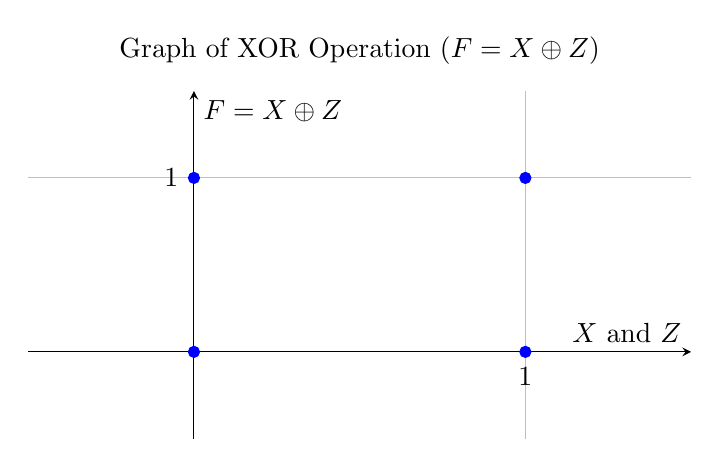
\begin{tikzpicture}
        \begin{axis}[
            axis lines = middle,
            xlabel = {$X$ and $Z$},
            ylabel = {$F = X \oplus Z$},
            xmin=-0.5, xmax=1.5,
            ymin=-0.5, ymax=1.5,
            xtick={0, 1},
            ytick={0, 1},
            width=10cm,
            height=6cm,
            grid=both,
            title={Graph of XOR Operation ($F = X \oplus Z$)}
        ]
        % Data points for XOR Truth Table
        \addplot[only marks, blue] coordinates {(0,0) (0,1) (1,1) (1,0)};
        \end{axis}
    \end{tikzpicture}
    \caption{Graph of XOR Logic ($F = X \oplus Z$)}
\end{figure}

\vspace{0.5cm}

\Large{\textbf{\textcolor{blue}{Final Answer: (D)  $Z = 0$}}}

\end{document}
